\documentclass[11pt, dvipsnames, DIV=12]{scrreprt}
\usepackage{babel}

\usepackage[utf8]{inputenc}
\usepackage[T1]{fontenc}
\usepackage{natbib}
\bibliographystyle{abbrvnat}
\usepackage{subcaption}
\usepackage{booktabs}
\usepackage{multirow}
\usepackage{url}
\usepackage{tikz}
\usepackage{paralist}

\usepackage{ifthen}
\newcommand{\CC}[1][]{$\text{C\hspace{-.25ex}}^{_{_{_{++}}}}
\ifthenelse{\equal{#1}{}}{}{\text{\hspace{-.625ex}#1}}$}

\usepackage{bm}
\usepackage{amsmath}
\usepackage{amssymb}
\usepackage{amsthm}
\usepackage{amsfonts}
\usepackage{thmtools}		
\usepackage{mleftright}
\usepackage{stmaryrd}
\usepackage{nicefrac}
\usepackage{algorithm}
\usepackage{algorithmicx}
\usepackage[noend]{algpseudocode}
\renewcommand{\algorithmicrequire}{\textbf{Input:}}
\renewcommand{\algorithmicensure}{\textbf{Output:}}

% Fixes some spacing issues with braces.
\let\originalleft\left
\let\originalright\right
\renewcommand{\left}{\mathopen{}\mathclose\bgroup\originalleft}
\renewcommand{\right}{\aftergroup\egroup\originalright}

\theoremstyle{definition}
\newtheorem{theorem}{Theorem}
\newtheorem{conjecture}{Conjecture}
\newtheorem{proposition}[theorem]{Proposition}
\newtheorem{insight}{Insight}
\newtheorem{observation}{Observation}
\newtheorem{lemma}[theorem]{Lemma}
\newtheorem{corollary}[theorem]{Corollary}
\newtheorem{definition}[theorem]{Definition}
\newtheorem{example}[theorem]{Example}
\newtheorem{remark}[theorem]{Remark}
\newtheorem{claim}[theorem]{Claim}
\newtheorem{fact}[theorem]{Fact}
\usepackage{thm-restate}
\usepackage[mathic=true]{mathtools}
\usepackage{fixmath}
\usepackage{siunitx}

\usepackage{pifont}
\newcommand{\cmark}{\ding{51}}
\newcommand{\xmark}{\ding{55}}
\usepackage{blindtext}

\usepackage{todonotes}

\usepackage{enumitem}
\setlist[enumerate]{itemsep=0.2ex, topsep=0.5\topsep}
\setlist[description]{itemsep=0.2ex, topsep=0.5\topsep}
\setlist[itemize]{itemsep=0.2ex, topsep=0.5\topsep}


% Let cleveref and thmtools work together
\makeatletter
\def\thmt@refnamewithcomma #1#2#3,#4,#5\@nil{%
\@xa\def\csname\thmt@envname #1utorefname\endcsname{#3}%
\ifcsname #2refname\endcsname
\csname #2refname\expandafter\endcsname\expandafter{\thmt@envname}{#3}{#4}%
\fi
}
\makeatother


\usepackage[pagebackref,
pdfa,
hidelinks,
pdftex, 
pdfdisplaydoctitle,
pdfpagelabels,
pdfauthor={},
pdftitle={},
pdfsubject={},
pdfkeywords={},
pdfproducer={Latex with the hyperref package},
pdfcreator={pdflatex}
]{hyperref}

\usepackage[capitalise,noabbrev]{cleveref}   

\usepackage{microtype}
\usepackage{ellipsis}

\usepackage[scaled=0.86]{helvet}
\usepackage{lmodern}

% Bold. 
\newcommand{\mF}{\mathbf{F}}
\newcommand{\mG}{\mathbf{G}}
\newcommand{\mH}{\mathbf{H}}
\newcommand{\mL}{\mathbf{L}}
\newcommand{\mI}{\mathbf{I}}

\newcommand{\mW}{\mathbf{W}}
\newcommand{\ma}{\mathbf{a}}
\newcommand{\mb}{\mathbf{b}}
\newcommand{\mw}{\mathbf{w}}

\newcommand{\ba}{\ensuremath{{\bf a}}}
\newcommand{\bb}{\ensuremath{{\bf b}}}
\newcommand{\bc}{\ensuremath{{\bf c}}}

% Calligraphic.
\newcommand{\cC}{\mathcal{C}}
\newcommand{\cF}{\mathcal{F}}
\newcommand{\cG}{\mathcal{G}}
\newcommand{\cH}{\mathcal{H}}
\newcommand{\cN}{\mathcal{N}}
\newcommand{\cO}{\mathcal{O}}
\newcommand{\cP}{\mathcal{P}}
\newcommand{\cR}{\mathcal{R}}
\newcommand{\cS}{\mathcal{S}}
\newcommand{\cT}{\mathcal{T}}
\newcommand{\cU}{\mathcal{U}}
\newcommand{\cV}{\mathcal{V}}

% Sans serif.
\newcommand{\sC}{\mathsf{C}}

% Blackboard.
\newcommand{\Fb}{\mathbb{F}}
\newcommand{\Gb}{\mathbb{G}}
\newcommand{\Nb}{\mathbb{N}}
\newcommand{\Qb}{\mathbb{Q}}
\newcommand{\Rb}{\mathbb{R}}
\newcommand{\Zb}{\mathbb{Z}}

% Multiset Definition
\newcommand{\MSopen}{\{\!\!\{}
\newcommand{\MSclose}{\}\!\!\}}

\usetikzlibrary{calc}


\usepackage[auth-lg]{authblk}
\newcommand{\cm}[1]{{{\textcolor{purple}{\textbf{[CM:} {#1}\textbf{]}}}}}


\renewcommand*{\Affilfont}{\large\normalfont}
\renewcommand*{\Authfont}{\normalfont}

\recalctypearea
\setcounter{Maxaffil}{2}

\title{\emph{On the theoretical equivalence of 1-WL+NN and GNNs and an empirical study on their performances}\\
\vspace{20pt}\small{\normalfont From the faculty of Mathematics, Physics, and Computer Science for the purpose of obtaining the academic degree of Bachelor of Sciences.}
}
\author{Eric Tillmann Bill}
\affil{\vspace{100pt}}

\author{Supervision:\\Prof. Dr. rer. nat. Christopher Morris}
\affil{Informatik 6\\RWTH Aachen University}

\date{\vspace{-30pt}}

\renewcommand{\thesection}{\arabic{section}}

\begin{document}

\maketitle
\tableofcontents

\section{Abstract}


\section{Introduction}
\begin{itemize}
    \item Teaser the reader why graphs are important, how neural networks in general have a significant impact on machine learning up to this day, and conclude that Graph Neural Networks are very interesting as they provide a trainable framework for classification on graphs, similar to ANNs or CNNS.\\
    Possible applications: Computer progamms, Semantic Web, Chemoinformatics, computer vision and graphics, graph matching, \cite{Morris2021}.
    \item Shortly outline the difficulties graphs are introducing compared to data ANNs or CNNs are working on (like regression, images) and explain how crucial it is to stay general in the approach as we can make no assumptions about the structure of the graphs.
    \item Introduce Weisfeller and Lehman\footnote{Based on https://www.iti.zcu.cz/wl2018/pdf/leman.pdf, we will use the spelling "Leman" here, as requested by A. Leman, the co-inventor of the algorithm.} and their 1-WL algorithm, by only mentioning how it recolors every node in every iteration based on each node's and neighbor's node's colors. Thereby effectively encoding information about the substructure each node of the graph is contained in.
    \item Teaser how GNNs in their most common architecture (message passing) somehow do the same and that between the 1-WL and GNNs are a couple of similarities, like for example that it has been shown that every GNN is at most as powerful in determining the Isomorphic Problem on graphs as the 1-WL algorithm.
    \item Introduce the main topic of the thesis, the first more theoretical part of this thesis will try that the 1-WL algorithm combined with Neural Networks are capable of computing every function that is computable by a GNN. Therefore, showing that 1-WL + NN are equivalent to GNN in their expressiveness. The second part will investigate emprically which encoding of the features space for 1-WL works best and more importantly how 1-WL + NN compared to GNNs are generalizing their task.
\end{itemize}

\section{Related Work}
\subsection{Graph Neural Networks}
In recent years, machine learning models have experienced a surge in popularity due to their significant performance advantages over conventional methods and their ability to autonomously adapt to their task. However, a closer examination of the applications where these models have been used reveals that they are highly specialized for the specific input of each application. For instance, modern convolutional neural networks are designed to take in fixed, grid-like data structures such as images, while modern language models process sequential data like text.

The relevance of graphs to these examples lies in the fact that graphs can be used to model all types of inputs in various applications, and they provide a more general framework for modeling data. To illustrate, an image can be modeled as a graph for a CNN, where each pixel corresponds to a node in the graph holding the brightness value for each color value, and each node is connected to its neighboring pixels. Similarly, for sequential data, one can encode a directed graph where each word is represented as a node with the word as a feature, and it is connected outgoingly to the next following word. With these examples, we wanted to highlight the flexibility of how graphs can model data, however, this is also problematic, as this makes it particularly hard to construct a general machine-learning model on graphs. Levering any constraints on the format or size of the input can significantly limit the models generality, and since graphs sizes and formats can vary within the application, e.g. chemical molecule classifyng, the need for a general model is of great interest.

From the work of \cite{Gil+2017}, as well \cite{Sca+2009}, the so called message-passing architecture emerged for Graph Neural Networks (short GNNs). This can be understood as a framework that never changes its input graph structurally and only modifies the node's features in each layer. In more detail, in each layer, a GNN based on the message-passing architecture, computes for each node a new feature, based on its previous feature and the features of its neighbors. Later in section \ref{sec:GNN Defintion}, we will give a more formal definition of this architecture.

TODO:
Although there have also been other frameworks proposed like the work of Tönshoff et al which uses random walks, or more powerful modifications like Li et al 2016 that uses a distance information, the message-passing architecture seems to be the most promising, as many researchers focus on it. 

Throughout this thesis, I will use the term GNN and message-passing architecture interchangeably.


\subsection{Weisfeiler and Leman Algorithm}
The (1-dimensional) Weisfeiler-Leman algorithm (short 1-WL), proposed by \cite{Wei+1968}, was initially designed as a simple heuristic for the \textit{graph isomorphism problem}, but due to its interesting properties and simplicity it is now used among other things as a graph kernel in GNNs, for example, \cite{She+2009b, She+2011}. One of these properties is, that the algorithm color codes the nodes of the input graph in such a way, that each color of a node encodes a local substructure the node is contained in, in each iteration.

It works by coloring all nodes in each iteration equally that already are colored the same and the frequencies of the colors of their neighbors are equal. The algorithm continues as long as the number of colors changes until the coloring is stable. In determining whether two graphs are non-isomorphic, the heuristic would apply the algorithm to both graphs simultaneously and conclude that the graphs are non-isomorphic as soon as the number of occurrences of a color is different between the graphs. We present a more formal definition of the algorithm later in the section \ref{sec:1-WL Definition}.

Since the \textit{graph isomorphism problem} is difficult to solve due to it being \textsf{NP}\textit{-complete}, the 1-WL algorithm, running in polynomial deterministic time, cannot solve the problem completely. Moreover, \cite{Cai1992} have constructed counterexamples for non-isomorphic graphs that the heuristic fails to distinguish, e.g. figure \ref{1-WL Counter Example}. However, following the work of \cite{Bab+1979}, this simple heuristic is still quite powerful and has a very low probability of failing to distinguish non-isomorphic graphs when both graphs are uniformly chosen at random.

To overcome the limited expressiveness of the 1-WL algorithm, it was generalized to the k-dimensional Weisfeiler-Leman algorithm (short $k$-WL), which works with $k$-tuples over the set of nodes instead of nodes. Interestingly, this created a hierarchy for the expressiveness of determining non-isomorphism, such that for all $k \in \mathbb{N}$ there exists a pair of non-isomorphic graphs that can be distinguished by the $(k+1)$-WL but not by the $k$-WL (\cite{Cai1992}).

\subsection{Connections between GNNs and the WL algorithm}
A connection between GNNs based on the message-passing architecture and the 1-WL algorithm seems quite natural since both share similar properties in terms of how they process graph data. Most noticeably, both methods never change the graph structurally, since they only compute new node features in each iteration. And in more detail, both methods use a 1-hop neighborhood aggregation as their basis for the computation of the new node feature. Following this intuition, many authors showed a theoretical connection between these methods. \cite{Morris2018}, as well as \cite{Xu2018}, showed that GNN's expressiveness power is upper bounded by the 1-WL in terms of distinguishing non-isomorphic graphs. In Addition, \cite{Morris2018} also proposed a new $k$-GNN architecture that works over the set of subgraphs of size $k$. Interestingly, the authors showed that the proposed hierarchy over $k \in \mathbb{N}$ is equivalent to the $k$-WL hierarchy in terms of their expressive in distinguishing non-isomorphic graphs, meaning if there exists a $k$-GNN that can distinguish two non-isomorphic graphs than it is equivalent to say that the $k$-WL algorithm can distinguish these graphs as well.

\section{Preliminaries}
We first introduce a couple of notations that will be used in this thesis. With $[n]$ we denote the set $\{1, \ldots, n\} \subset \mathbb{N}$ for any $n \in \mathbb{N}$ and for $\MSopen \ldots \MSclose$ we denote a multiset which is formally defined as a 2 tuple $(X, m)$ with $X$ being a set of all unique elements and $m: X \rightarrow \mathbb{N}_{\geq 1}$ a mapping that maps every element in $X$ to its number of occurrences in the multiset.

\subsection{Graph Framework}
A graph is denoted by $G$ and is a 3 tuple $G:= (V, E, l)$ that consists of the set of all nodes $V$, the set of all edges $E \subseteq V \times V$ and a label function $l: M \rightarrow \Sigma$ with $M$ being either $V, V \cup E$ or $E$ and $\Sigma \subset \mathbb{N}$ a finite alphabet. Moreover, let $\mathcal{G}$ be the set of all graphs. Note, that our definition of the label function allows for graphs with labels either only on the nodes, only on the edges, or on both nodes and edges. In addition, although we have defined it this way, the labeling function is optional, and in cases where no labeling function is given, we add the trivial labeling function $f_0: V(G) \rightarrow \{0\}$. Further, $G$ can be either directed or undirected, depending on the definition of $E$, where $E \subseteq \{(v,u) \mid v,u \in V\}$ defines a directed and $E \subseteq \{(v, u), (u,v) \mid v,u \in V, v\neq u\}$ defines an undirected graph. Additionally, we will use the notation $V(G)$ and $E(G)$ to denote the set of nodes of $G$ and the set of edges of $G$ respectively. With $\mathcal{N}(v)$ for $v \in V(G)$ we denote the set of neighbors of $v$ with $\mathcal{N}(v) := \{u \mid (u, v) \in E(G)\}$

\subsection{Permutation-invariance and -equivariance}
We use $S_n$ to denote the symmetric group over the elements $[n]$ for any $n > 0$. $S_n$ consists of all permutations over these elements. Let G be a graph with $V(G) = [n]$, applying a permutation $\pi \in S_n$ on G, is defined as $G_\pi := \pi \cdot G$ where $V(G_\pi) = \{\pi(1), \ldots, \pi(n) \}$ and $E(G_\pi) = \{ (\pi(v), \pi(u)) \mid (v,u) \in E(G)\}$. We will now introduce two key concepts for classifying functions on graphs. Let $f: \mathcal{G} \rightarrow \mathcal{X}$ be an arbitrary function and let $V(G) = [n_G]$ where $n_G := |V(G)|$ for every $G \in \mathcal{G}$:\\
\noindent The function $f$ is \textit{permutation-invariant} if and only if for all $G \in \mathcal{G}$ where $n_G := \mid V(G) \mid$ and for every $\pi \in S_{n_G}$: $f(G) = f(\pi \cdot G)$.\\
\noindent The function $f$ is \textit{permuation-equivariant} if and only if for all $G \in \mathcal{G}$ where $n_G := \mid V(G) \mid$ and for every $\pi \in S_{n_G}$: $f(G) = \pi^{-1} \cdot f(\pi \cdot G)$.

TODO: Mention that those definitions are adapted and inspired by \cite{Morris2021}.

\subsection{Weisfeiler and Leman Algorithm}\label{sec:1-WL Definition}
We work here with a combination of the original Weisfeiler and Leman Algorithm and the color refinement algorithm which we call in general 1-dimensional Weisfeiler and Leman algorithm (short 1-WL). TODO: check the statement and add citations.

Let $G = (V,E,l)$ be a graph, then in each iteration $i$, the 1-WL computes a node coloring $C_i: V(G) \rightarrow \mathbb{N}$, which depends on the coloring of the neighbors and the node itself. In iteration $i=0$, the initial coloring is $C_0 = l$ or if $l$ is non existing $C_0 = c$ for an arbitrary constant $c \in \mathbb{N}$. For $i > 0$, the algorithm assigns a color to $v \in V(G)$ as follows:
\begin{align*}
C_i (v) = \textsf{RELABEL}((C_{i-1}(v), \MSopen C_{i-1}(u) \mid u \in \mathcal{N}(v) \MSclose))
\end{align*}

\noindent Where $\textsf{RELABEL}$ injectively maps the above pair to a unique, previously not used, natural number. The algorithm terminates when the number of colors between two iterations does not change, meaning the algorithm terminates after iteration $i$ if the following condition is satisfied:
\begin{align}
\forall v,w \in V(G):  C_i(v) = C_i(w) \iff C_{i+1}(v) = C_{i+1}(w)
\end{align}
Upon terminating we define $C_{\infty}$:= $C_i$ as the stable coloring. Note that the algorithm always terminates after $n_G := |V(G)|$ iterations as there are only $n_G$ different cardinalities of the image under any coloring. TODO: check the reasoning, I think $|C_i|$ <$|C_{i-1}|$ but have no recollection of this.

To determine if two graphs $G, H \in \mathcal{G}$ are non-isomorphic (short $G \ncong H)$, one would apply the 1-WL algorithm on both graphs "in parallel" and check after each iteration if the occurrences of each color are equal, else the algorithm would terminate and conclude non-isomorphic. Formally, the algorithm concludes non-isomorphic in iteration $i$ if there exists a color $c$ such that: $|\{ v \in V(G) \mid c = C_i(v)\} | \neq |\{ v \in V(H) \mid c = C_i(v)\} |$. Note that this method is only sound and not complete for the problem of graph isomorphism. Counterexamples where the algorithm fails to distinguish non-isomorphic graphs can be easily constructed, see Figure \Ref{1-WL Counter Example} which was discovered and proven by \cite{Cai1992}.

\begin{figure}[H]
    \centering
    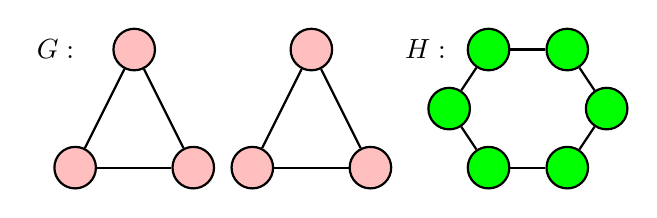
\begin{tikzpicture}

\tikzset{line/.style={draw,thick}}
\tikzset{arrow/.style={line,->,>=stealth}}
\tikzset{node/.style={circle,inner sep=0pt,minimum width=15pt}}

\draw (-1.0,0.75) node {$G:$};
\node[line,node,fill=pink] (x1) at (0, 0.75) {};
\node[line,node,fill=pink] (x2) at (-0.75, -0.75) {};
\node[line,node,fill=pink] (x3) at (0.75, -0.75) {};

\path[line] (x1) to (x2);
\path[line] (x1) to (x3);
\path[line] (x2) to (x3);

\node[line,node,fill=pink] (x1) at (2.25, 0.75) {};
\node[line,node,fill=pink] (x2) at (1.5, -0.75) {};
\node[line,node,fill=pink] (x3) at (3.0, -0.75) {};

\path[line] (x1) to (x2);
\path[line] (x1) to (x3);
\path[line] (x2) to (x3);

\draw (3.7, 0.75) node {$H:$};
\node[line,node,fill=green] (x1) at (3.75 + 0.25, 0) {};
\node[line,node,fill=green] (x2) at (4.25 + 0.25, 0.75) {};
\node[line,node,fill=green] (x3) at (5.25 + 0.25, 0.75) {};
\node[line,node,fill=green] (x4) at (5.75 + 0.25, 0) {};
\node[line,node,fill=green] (x5) at (5.25 + 0.25, -0.75) {};
\node[line,node,fill=green] (x6) at (4.25 + 0.25, -0.75) {};

\path[line] (x1) to (x2);
\path[line] (x2) to (x3);
\path[line] (x3) to (x4);
\path[line] (x4) to (x5);
\path[line] (x5) to (x6);
\path[line] (x6) to (x1);

\end{tikzpicture}
    \caption{An example of two graphs $G$ and $H$ that are non-isomorphic but cannot be distinguished by the 1-WL}
    \label{1-WL Counter Example}
\end{figure}

\subsection{1-WL+NN Framework}\label{sec:1-WL+NN Definition}
Let $\mathcal{Y}$ be the task-specific output set (e.g. set of class labels), $\mathcal{NN}$ a feedforward neural network, $\textsf{enc}$ an encoding function, $\pi_{pool}$ a pooling function. Further, for $G \in \mathcal{G}$, let $(C^i_\infty)_{G}$ be the final coloring upon termination when applying the 1-WL algorithm on $G$. Than the computed function $\mathcal{A}$ is:
\begin{align}
\mathcal{A}: \mathcal{X} \rightarrow \Sigma, \  G \mapsto \mathcal{NN} \circ \pi_{pool}(\MSopen (C^i_\infty)_{G}(v) \mid v \in V(G) \MSclose)
\end{align}

\subsection{Graph Neural Networks (Message Passing)}\label{sec:GNN Defintion}
Let $G = (V, E, l)$ be an arbitrary graph. A Graph Neural Network (GNN) is a composition of multiple layers where each layer $t$ passes a vector representation of each node $v$ or edge $e$ through $f^{(t)}(v)$ or $f^{(t)}(e)$ respectively and retrieves thereby a new graph that is structurally identical but has new label information. To begin with, we need a function $f^{(0)}: V(G) \rightarrow \mathbb{R}^{1 \times d}$ that is consistent with $l$, that translates all labels into a vector representation. Further, for every $t > 0$, $f$ is of the format:
\begin{align}
f^{(t)}(v) = f^{W_{1,t}}_{merge} (f^{(t-1)}(v), \  f^{W_{2,t}}_{agg}( \MSopen f^{(t-1)}(w) \mid w \in \mathcal{N}(v) \MSclose ))
\end{align}

\noindent Where $f^{W_{1,t}}_{merge}$ and $f^{W_{2,t}}_{agg}$ are arbitrary differentiable functions with $W_{1,t}$ and $W_{2,t}$ their respective parameters. Additionally, $f^{W_{2,t}}_{agg}$ has to be permuation-invariant. This definition has been adapted from \cite{Morris2018}.

\noindent Depending on the objective, whether the GNN is tasked with node classification or graph classification, the last layer differs. In the latter case, we add a permutation-invariant aggregation function to the end, here called $\textsf{READOUT}$, that aggregates over every node and computes a single label for the entire graph (inspired by \cite{Xu2018}). Note, in order to ensure that we can train the GNN in an end-to-end fashion, we require $\textsf{READOUT}$ to be also differentiable.

Let $\mathcal{A}$ be an instance of the described GNN framework. Further, let $K \in \mathbb{N}$ be the number of layers of the GNN, $\mathcal{G}$ the set of all graphs, $\mathcal{Y}$ the task-specific output set (e.g. labels of a classification task), then the overall function computed by $\mathcal{A}$ is:
\begin{align}
&\mathcal{A}: \mathcal{G} \rightarrow \mathcal{Y}: x \mapsto \circ f^{(K)} \circ \ldots \circ f^{(0)}(x)\\
&\mathcal{A}: \mathcal{G} \rightarrow \mathcal{Y}: x \mapsto \textsf{READOUT} \circ f^{(K)} \circ \ldots \circ f^{(0)}(x)
\end{align}
As we required all aggregation functions to be permutation-invariant, the total composition $\mathcal{A}$ is permutation-invariant, and similarly, it is also differentiable. This enables us to train $\mathcal{A}$ like any other machine learning method in an end-to-end fashion, regardless of the underlying encoding used for graphs.


\section{Main Part}
\subsection{Theoretical Part}
\begin{itemize}
    \item Proof of the following statement: "Every function computed by a GNN, can also be computed 1-WL+NN. The GNN is defined as in section \ref{sec:GNN Defintion} and the 1-WL+NN as in section \ref{sec:1-WL+NN Definition}."
    \item Idea for now is that one can connect the functions computable by 1-WL+NN to a class that is universally approximating. From this on I will show that this class is equivalent to all functions computable by a GNN. 
\end{itemize}

\subsection{Emprical / Practical Part}
\begin{itemize}
    \item Elaborate on the datasets I want to use? Why these, their related fields, and related work already conducted on them and why it is particularly good to use them
    \item As baseline use the implementation GCN(Kipf & welling 2017), GraphSAGE(Hamilton 2017) and GIN(Xu2018)
\end{itemize}
\subsubsection{Encoding}
\begin{itemize}
    \item For the different embedding schemas used for the 1-WL algorithm, I want to consider: 1. one-hot encoding 2. Look up Table 3. GNNs
    \item Explain that I will implement all these solutions by using the state-of-the-art implementations of Pytorch and the opensource extension for graphs Pytorch\_geometric
    \item State a hypothesis that I think that the 2. or 3. option will have a significant difference in performance in comparison to option 1.
    \item State how I will evaluate these results. Mentioning the statistical tools I am going to use
\end{itemize}

\subsubsection{1-WL vs GNNs}
\begin{itemize}
    \item Test all models, including all encoding variants of the previous section on the selected datasets.
\end{itemize}

\setcitestyle{numbers}
\bibliography{references}
\end{document}
